\documentclass{article}
\usepackage{graphicx} % Required for inserting images
\usepackage[dvipsnames]{xcolor}
\usepackage{multirow,array}
\usepackage{float}
\usepackage[spanish]{babel}
\usepackage{amsmath}

\newcommand{\stratU}[1]{\textbf{\textcolor{RoyalBlue}{#1}}}
\newcommand{\stratD}[1]{\textbf{\textcolor{RedOrange}{#1}}}
\newcommand{\strat}[2]{(\stratU{#1}, \stratD{#2})}
\newcommand{\stratPay}[2]{(\textcolor{RoyalBlue}{#1}, \textcolor{RedOrange}{#2})}

\title{Teoría de Juegos}
\author{Ejercicio Modelado}
\date{28/4/2023}

\begin{document}

\maketitle

\section*{Integrantes}

\begin{itemize}
    \item Manuel Panichelli, L.U. 72/18
    \item Ignacio Alonso Rehor, L.U. 195/18
\end{itemize}

\section*{Enunciado}

Elegir una idea o situación de la vida real (comercial, social, académica o laboral), distinta de las vistas, y modelarla como un juego en forma normal entre n personas (para algún n fijo). Para esta situación, mostrar cuáles son los jugadores y todo lo necesario para tener un juego en forma normal. Indicar justificando si este es finito, si es de suma cero y si es de información perfecta. Mostrar situaciones de ejemplo sobre el mismo. Determinar/discutir la existencia de equilibrios de Nash puros. Si se aplica y está definido, determinar el valor inferior, el valor superior y el valor puro.

\section*{Introducción}

La situación que elegimos para modelar, \textbf{Rebase}, consiste en lo siguiente: Un conductor intenta rebasar a un camión en la ruta cuando se encuentra que se aproxima un auto en la mano contraria. Además, ambos conductores deducen que el rebase no se podrá completar antes de chocar. Luego, ambos deberán decidir cómo evitar el accidente.

\begin{figure}[H]
    \centering
    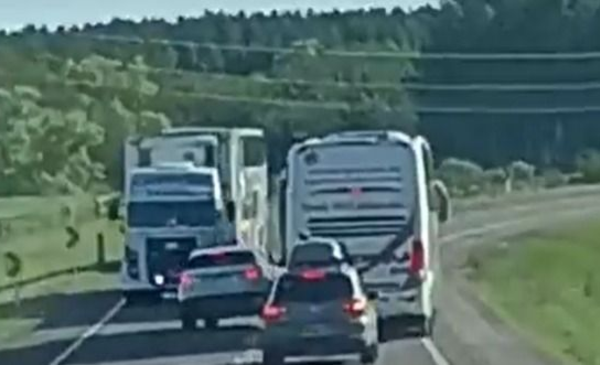
\includegraphics[scale=0.5]{rebase.png}
    \caption{Un auto intenta rebasar a un camión, pero se da cuenta que no llega}
\end{figure}

\section*{Definiciones}

El juego será

$$G = (I, S, u)$$

donde

\begin{itemize}
    \item $I = \{ J_1, J_2 \}$ son los jugadores
    \item $S = \{ S_1, S_2 \}$ son las estrategias
    \item $u = (u_1, u_2)$ son las funciones de pago
\end{itemize}


El jugador $J_1$ será el que intenta rebasar y $J_2$ el de la mano contraria.

Las posibles estrategias de $J_1$ son:

\begin{itemize}
 \item \stratU{volver}: Decide no continuar con el rebase y vuelve a su posición detrás del camión a la espera de otro momento para pasarlo.
 
 \item \stratU{seguir}: Decidido a rebasar al camión, opta por no cambiar de rumbo y pisar el acelerador.
 
 \item \stratU{banquina}: Temiendo lo que pueda llegar a hacer el otro auto, decide tirarse a la banquina del otro carril.

\end{itemize}

En cambio, para el jugador $J_2$, sus posibles estrategias son:

\begin{itemize}
    \item \stratD{banquina}: Opta por quitarse del camino del otro conductor tirandose a su banquina.
    \item \stratD{seguir}: Confía en el criterio del otro conductor y sigue por el mismo camino que venía.
    
\end{itemize}

Luego las estrategias conjuntas serán,

\begin{itemize}
    \item \strat{seguir}{seguir}: chocan. $J_1$ se verá más perjudicado que el segundo porque al ser el el que estaba rebasando, no lo cubre el seguro.
    \item \strat{seguir}{banquina}: $J_1$ se ve beneficiado porque llega antes a su destino, mientras que $J_2$ perjudicado porque se daña su auto al tirarse a gran velocidad a la banquina.
    \item \strat{volver}{seguir}: evitan la colisión, y se ve perjudicado $J_1$ porque tarda más en llegar a su destino.
    \item \strat{volver}{banquina}: ambos se ven perjudicados. $J_2$ daña su auto al ir a la banquina y $J_1$ tarda más en llegar a su destino.
    \item \strat{banquina}{seguir}: $J_1$ se ve perjudicado ya que su auto se daña en la banquina y además va a tardar más en volver a su carril porque tiene que esperar a que no pasen más autos.
    \item \strat{banquina}{banquina}: también chocan.
\end{itemize}

$u$ está dada por la siguiente matriz de pagos
% Considerar https://www.economics.utoronto.ca/osborne/latex/sgame.pdf
\begin{center}
    \begin{table}[H]
    \setlength{\extrarowheight}{2pt}
    \begin{tabular}{cc|c|c|}
      & \multicolumn{1}{c}{} & \multicolumn{2}{c}{\stratD{Jugador 2}}\\
      & \multicolumn{1}{c}{} & \multicolumn{1}{c}{\stratD{seguir}}  & \multicolumn{1}{c}{\stratD{banquina}} \\\cline{3-4}
      \multirow{3}*{\stratU{Jugador 1}}  & \stratU{seguir} & $\stratPay{-5}{-4}$ & $\stratPay{1}{-2}$ \\\cline{3-4}
        & \stratU{volver} & $\stratPay{-1}{0}$ & $\stratPay{-1}{-2}$ \\\cline{3-4}
        & \stratU{banquina} & $\stratPay{-3}{0}$ & $\stratPay{-5}{-4}$ \\ \cline{3-4}
    \end{tabular}
    \end{table}
\end{center}

\section*{Análisis}

Algunas observaciones sobre el juego,

\begin{itemize}
    \item \textbf{No es de suma cero}. la función de pagos de $J_1$ no resulta opuesta a la del jugador $J_2$. En particular,
    \[
        u_1(\text{volver}, \text{seguir}) + u_2(\text{volver}, \text{seguir})
        = -1 + 0 = -1 \neq 0
    \]

    \textit{Por lo tanto, no vamos a hablar sobre los valores ya que no están definidos.}
    \item \textbf{Es finito} ya que $S_1$ y $S_2$ son finitos.
    \item \textbf{No es de información perfecta}. Si lo representáramos en forma extensiva, el jugador que le toque elegir segundo no podría saber que hizo el primero (ya que es una elección simultánea). Por lo tanto, su conjunto de información tendría 3 nodos, y al no ser unitario no es de información perfecta.
\end{itemize}

\subsection*{Equilibrios de Nash}

Podemos observar que para el jugador $J_1$ la estrategia \stratU{banquina} \textbf{está dominada} por las otras dos. Esto significa que, si el jugador $J_1$ es un agente racional (que es debatible dado las condiciones del problema), este nunca debería optar por esta estrategia. Esto se debe a que la estrategia \stratU{volver} garantiza un pago estrictamente mayor para cualquier elección de estrategia del jugador $J_2$.

También podemos ver que las estrategias conjuntas \strat{seguir}{banquina} y \strat{volver}{seguir} resultan dos \textbf{equilibrios de Nash}. Esto es porque, si en algún momento se llega a este estado, el pago de ambos jugadores se vería disminuido si cualquiera de estos dos variara su elección de estrategia.

\section*{Conclusiones}

\begin{itemize}
    \item  Esta manera de modelar esta situación de la vida cotidiana termina siendo un poco reduccionista por dos puntos fundamentales:

\begin{enumerate}
    \item Estamos suponiendo que ambos jugadores tienen absoluta certeza de que no se puede completar el rebase. Esto en la vida real sería imposible de garantizar.
    \item El jugador $J_1$ siempre tiene la posibilidad de volver a la meterse detrás del camión. Pero en la vida real esta posibilidad puede no estar disponible si otro auto ocupó su lugar.
\end{enumerate}

 No obstante, este modelo nos brinda un resultado interesante: al conductor intentando rebasar nunca le conviene tirarse a la banquina del carril contrario.

\item Así mismo, el juego que resulta de eliminar la estrategia dominada \stratU{banquina} es muy parecido a \textbf{Gallina}. La situación modelada es similar y ambos tienen dos equilibrios de Nash cuando sus estrategias son opuestas.

\end{itemize}
\end{document}
